\section{Formalism}
\label{sec:formalism}

This section provides a formal model of our universe in~\cref{sec:universe} and
formalizes the Improvement Game in \cref{sec:improvement}. \Cref{sec:potential}
defines potential, and the important concepts of horizons in~\cref{sec:horizon}
and fairness in~\cref{sec:fairness}. We conclude this section by proving
theorems of stability in~\cref{sec:stability}.

\subsection{The Universe Model}
\label{sec:universe}

To investigate the concept of potential
maximization, we model the universe as a tuple $(X, U, u_0, A, t, r)$.
\begin{itemize}
  \item $X$ is the set of classes, each associated with a decision-making
        strategy.
  \item $U$ is the set of states that the universe can be in.
  \item $u_0 \in U$ is the initial state of the universe.
  \item $A_{x, u}$ is the set of actions from which the class $x \in X$ can
        choose in state $u \in U$.
  \item $t(u, a) \in U$ is the transition function, which takes the universe's
        current state $u \in U$, along with actions $a$ for each class, and
        returns the universe's next state. $a$ is modeled as a function that
        maps every class $x \in X$ to its chosen action $a(x) \in A_{x,u}$.
  \item $r(x, u) : \mathbb{R}$ is the reward function, which indicates how well
        class $x \in X$ is doing in the state $u \in U$.
\end{itemize}

We also require a number of technical side conditions, namely that rewards be
non-negative, that the set of classes be finite, that equality between classes
be decidable, and that any set of actions be finite and non-empty.

An instantiation of this model can be as simple as the Improvement Game
(defined in the next section) or as complex as the physical universe, where the
states $U$ represent the physical configuration of the universe, $t$ transitions
it according to the laws of physics, and $A$ is the set of actions available to
all agents executing $x$'s strategy.

We will regularly use the following definitions. The \emph{strategy} of a class
$x$ is given by a function $s(u) \in A_{x,u}$, which maps every state of the
universe $u \in U$ to the action chosen by the strategy in that state. We
represent the \emph{set of strategies} for every class $x \in X$ as a function
$S$, where $S(x,u) \in A_{x,u}$. We write $S[x = s]$ to represent the
strategies that are equal to $S$, except that the strategy for $x$ has been
replaced with $s$. Given $x$, the \emph{other strategies} $S$ refers to a set
of strategies for every $x' \neq x$.

Given a set of strategies $S$, we can then take one step of the universe from
$u$ to $u'$ by first defining the actions $a(x) = S(x,u)$ and then passing them
to the transition function $u' = t(u, a)$. We can iterate this relation starting
with $u$ to move the universe forward by any number of steps $n$, which we write
as $u_n = t_n(S,u)$. We simply write $t_n(S)$ when $u = u_0$.

\subsection{The Improvement Game}
\label{sec:improvement}

To better understand such potential maximization, we study the following simple game,
which we will call the \emph{Improvement Game}. In this game, a strategy
either makes an Improvement ($I$) or reaps its Reward ($R$). An Improvement creates no
immediate reward but increases the reward rate for future Reward
actions. A Reward action collects reward
according to the reward rate but keeps the reward rate unchanged.

Let us consider the resulting dynamics using the illustrations
in~\cref{fig:growth}. Compare the example strategy $X$, which always reaps its Reward,
with strategy $Y$, which makes 3 Improvements initially and then always
reaps its Reward. $X$ initially outperforms $Y$ but is then quickly overtaken by $Y$,
which has a higher reward rate. So while delaying reward collection to make
Improvements hurts in the short term, it is a better strategy in the long term.

Now consider strategy $Z$. This strategy only makes Improvements and never
reaps its Reward. This strategy is clearly bad at collecting rewards; in fact, it
never collects any reward. However, it also always has the highest
\emph{potential} to do so: if at any point it were to start using Reward
actions, it would quickly grow its cumulative reward and would eventually
outperform any other strategy.

\begin{figure}[!ht]
  \centering
  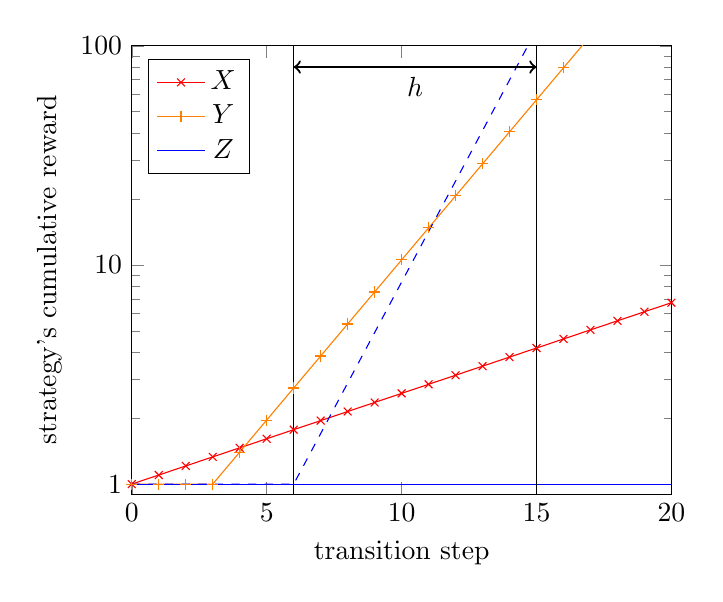
\begin{tikzpicture}
    \begin{axis}[
        xlabel={transition step},
        ylabel={strategy's cumulative reward},
        ymode=log,
        log ticks with fixed point,
        legend pos=north west,
        xmin=0, xmax=20,
        ymin=0.9, ymax=100,
        domain=0:20,
        samples=21
      ]
      \addplot[color=red, mark=x] expression {1.1^x};
      \addlegendentry{$X$}

      \addplot[color=orange, mark=+] expression {max(1, 1.4^(x - 3))};
      \addlegendentry{$Y$}

      \addplot[color=blue, mark=none] expression {1};
      \addlegendentry{$Z$}

      \addplot[color=blue, mark=none, dashed] expression {max(1, 1.7^(x - 6))};

      \draw[black] (axis cs:6, 0.9) -- (axis cs:6, 100);
      \draw[black] (axis cs:15, 0.9) -- (axis cs:15, 100);
      \draw[<->, black, thick] (axis cs:6, 80) -- (axis cs:15, 80) node[midway, below] {$h$};
    \end{axis}
  \end{tikzpicture}
  \caption{ Improvement Game strategy comparison. Strategy $X$ always
    reaps its Reward. It starts accumulating reward immediately, giving it a head start, but its
    reward rate is low, and so it is quickly overtaken by strategy $Y$, which
    starts with 3 Improvements to increase its reward rate and only then
    switches over to reaping its Reward. In general, strategies that make more
    Improvements before they reap their Reward always eventually outperform strategies
    with fewer Improvements --- the Improvement Game thus has no stable
    reward-maximizing strategies. Strategy $Z$ always makes Improvements and
    never reaps its Reward, which keeps its cumulative reward stuck at $1$. However, $Z$
    always has the highest \emph{potential} for reward maximization, meaning
    that at any point, if it were to start using Reward actions (indicated
    by the blue dashed line), it would quickly grow its cumulative reward and
    would eventually outperform any other strategy. We call the number of steps
    it takes to outperform any other strategy the horizon $h$. }
  \label{fig:growth}
\end{figure}

The Improvement Game has no evolutionarily stable strategy in terms of reward
collection, as any strategy can always be invaded by a strategy that performs more
Improvements. However, strategy Z, which always makes Improvements, is stable
and uninvadable in terms of its potential, despite being bad at actually
collecting any reward.

To formalize this game, we instantiate the universe as follows:

\begin{itemize}
  \item $X$ has just two members, $X = \{x_0, x_1\}$.
  \item $u \in U$ is a function that maps each class $x$ to a tuple $(m, f) =
          u(x)$, where $m \in \mathbb{R}$ is the cumulative reward of class
        $x$, and $f \in \mathbb{R}$ is $x$'s reward rate.
  \item $u_0(x) := (1, 1.1)$ sets the initial cumulative reward for each
        class to $1$ and the initial reward rate for each class to $1.1$.
  \item $A_{x, u} := \{I,R\}$ defines the actions a class can
        take. Either the class makes an Improvement ($I$),
        or it reaps its Reward ($R$).
  \item $t(u,a,x)$ updates $x$'s cumulative reward and reward rate
        according to the action $a$. Let $(m,f) = u(x)$. If $a(x) = I$, the
        transition function returns $(m,f + 0.1)$; and if $a(x) = R$, the
        transition function returns $(m \cdot f,f)$.
  \item $r(x, u)$ extracts the cumulative reward of $x$ from the
        universe state. The function returns $m$, where $(m, f) = u(x)$.
\end{itemize}

The tension in the Improvement Game is that Reward actions increase the reward
in the short term, while Improvements lead to higher rewards in the long term.
Because of this dynamic, no strategy is reward-maximizing at every step.

We say that a strategy $s$ is \emph{reward-maximizing} at $n$ for the class $x$,
with respect to the other strategies $S$, if and only if:

\begin{equation}
  \forall s', r (x, t_n(S[x=s])) \ge r (x, t_n(S[x=s']))
\end{equation}

\begin{theorem}
  In the Improvement Game, no strategy is reward-maximizing at every step.
\end{theorem}

\begin{proof}
  By contradiction. Assume there is a reward-maximizing strategy $s$ at every
  step. $s$ must execute a Reward action ($R$) for every step, because if it
  executed an Improvement action, another strategy could execute $R$ and achieve
  a higher reward for that step. The reward of $s$ at any step $n$ is thus
  $1.1^n$. Now consider a strategy $s'$ that first executes a single Improvement
  action and subsequently reaps its Reward. At step $n$, its reward will be
  $1.2^{n-1}$. At $n = 3$, the strategy $s'$ already has a higher reward than
  $s$, because $1.2^2 = 1.44 > 1.331 = 1.1^3$, which proves the contradiction.
\end{proof}

\subsection{Potential}
\label{sec:potential}

In the Improvement Game, a strategy that greedily maximizes the reward at every
step is unable to maximize the reward in the long term. Instead, let us consider
a strategy that maximizes the \emph{potential} $p$ for reward in the long term.

We define potential as the maximum reward that a given class could achieve in
$h$ steps from $u$, if that class could execute any strategy. We call $h$ the look-ahead value. Formally, we
define the potential $p$ for a given class $x$, other strategies $S$, and state
$u$ as follows. We omit the look-ahead $h$ when it is clear from the context.

\begin{equation}
  p_h(x,S,u) := \max_{s} \: r(x, t_h(S[x=s], u))
\end{equation}

In the state $u$, we define the action with the highest potential as the
\emph{potential-maximizing action} $a^*$:

\begin{equation}
  a^*_h(x,S,u) := (\argmax_{s} \: r(x, t_h(S[x=s], u)))(u)
\end{equation}

We define the highest potential reachable from state $u$ in $n$ steps as the
\emph{maximum potential} $p^*$, where we omit $u$ when $u = u_0$:

\begin{equation}
  p^*_h(x,S,n,u) := \max_{s} \: p_h(x, S, t_n(S[x=s], u))
\end{equation}

\subsubsection{Horizons}
\label{sec:horizon}

Potential is defined in terms of the look-ahead value, which specifies how far
into the future we look when evaluating potential. For short look-aheads, the
potential-maximizing action must work immediately toward increasing reward, so
it will reap its Reward ($R$). However, beyond a certain point $h$, there is
always enough time to maximize the reward later, and the
potential-maximizing action shifts to guiding the strategy onto a path with
more favorable outcomes---it starts making Improvements ($I$).

As we increase the look-ahead further beyond $h$, there is no further change in
the potential-maximizing action. We call an $h$ with this property a
\emph{horizon}. When a horizon exists, it becomes unnecessary to look beyond
that horizon, as it will not lead to a change in action. How long a horizon has
to be may depend on the number of transitions $n$ taken from the start state, so
we usually provide a family of horizons, indexed by the steps taken since $u_0$.

Formally, we consider a positive $h$ to be a horizon if for all $n$, classes
$x$, and strategies $S$, we have:

\begin{equation}
  \forall h' > {h_n}, a^*_{h_n}(x,S,t_n(S)) = a^*_{h'}(x,S,t_n(S))
\end{equation}

\begin{theorem}
  \label{lem:horizon-exists}
  In the Improvement Game, there exists a horizon $h_n$ for every $n$.
\end{theorem}

\begin{proof}
  See the appendix.
\end{proof}

When a horizon exists, we will usually omit the look-ahead when calling
functions like $p$ and pass the horizon implicitly.

\subsubsection{Fairness}
\label{sec:fairness}

We say that a universe is \emph{fair} if no class has an inherent
advantage in how quickly it can grow its potential---a class can only gain an
advantage by executing a better strategy. Formally, fairness means that
for all strategies $S$, classes $x$ and $x'$, and $n$, we have:

\begin{equation}
  \frac{p^*(x,S,n)}{p(x,S)} =
  \frac{p^*(x',S,n)}{p(x',S)}
\end{equation}

\begin{theorem}
  \label{lem:fairness}
  The Improvement Game is fair.
\end{theorem}

\begin{proof}
  We can rewrite any reward or potential as a product that contains no reference
  to $x$ (see \cref{lem:expo-seq} in the appendix), which makes the terms on
  both sides of the equation equal.
\end{proof}

Sometimes fairness is too strong an assumption. We therefore introduce a weaker
condition, \emph{economies of scale}, which is similar to fairness except that
classes with higher initial potential are permitted to grow their potential
faster than those with lower initial potential. Formally, for all strategies
$S$, classes $x$ and $x'$, and $n$, we have:

\begin{equation}
  p(x,S) \ge
  p(x',S) \rightarrow
  \frac{p^*(x,S,n)}{p(x,S)} \ge
  \frac{p^*(x',S,n)}{p(x',S)}
\end{equation}

\subsection{Stability}
\label{sec:stability}

Now that we have shown that the Improvement Game has horizons
(\cref{lem:horizon-exists}) and is fair (\cref{lem:fairness}), we can show that
a potential-maximizing strategy exists. In fact, we can show that such a
strategy exists not just in the Improvement Game but for \emph{any} universe
that has a horizon.

We say that a strategy $s$ is \emph{potential-maximizing} for the class $x$,
with respect to the other strategies $S$, if:

\begin{equation}
  \forall s' n, p(x, S, t_n(S[x=s])) \ge p(x, S, t_n(S[x=s']))
\end{equation}

\begin{theorem}
  \label{lem:potential-maximizing-strategy-ok}
  Any universe with a horizon has a potential-maximizing strategy
  $s^*$, for every class $x$ and other strategies $S$.
\end{theorem}

\begin{proof}
  Let $s^*(u) = a^*(x,S,u)$. We can rewrite the goal as $p(x,S,t_n(S[x=s^*],
    u_0)) = p^*(x,S,n,u_0)$. Generalize $u_0$ as $u$, then perform induction on
  $n$. The base case is trivial, as $p^*(x,S,0) = p(x,S,u_0)$. In the
  recursive case, we instantiate the induction hypothesis with $u' = t_1(S,
    u)$. $s^*$ executes the potential-maximizing action for the horizon at $u$,
  which by \cref{lem:horizon-exists} we can extend to the horizon at
  $t_n(S,u)$, so potential maximization $n+1$ steps from $u$ is possible, and
  by the induction hypothesis we know it is also taken.
\end{proof}

\begin{theorem}
  \label{lem:stability}
  If the universe is fair,
  a potential-maximizing strategy is \emph{stable}, in the sense that the
  strategy's share of potential, across all strategies, never decreases over
  time. Formally, for all $x$, other strategies $S'$, and $n$, where $S =
    S'[x = s^*(x,S')]$, and $u_n = t_n(S)$, we have:

  \begin{equation}
    \frac{p(x,S,u_n)}{\sum_{x'} p(x',S,u_n)} \ge \frac{p(x,S,u_0)}{\sum_{x'} p(x',S,u_0)}
  \end{equation}
\end{theorem}

\begin{proof}
  Because $x$ uses strategy $s^*$, we know by
  \cref{lem:potential-maximizing-strategy-ok} that $p(x,S,u_n)$ is equal to the
  maximum potential $p^*(x,S,n)$. We can also replace $p(x',S,u_n)$ in the denominator
  with the larger term $p^*(x',S,n)$, which by the fairness assumption, we
  can rewrite to $p(x',S,u_0) \frac{p^*(x,S,u_n)}{p(x,S,u_0)}$.
  This inequality is then trivially true.
\end{proof}

From \cref{lem:stability}, it trivially follows that a potential-maximizing
strategy's share cannot be invaded or replaced by a different strategy.

If we only have the weaker assumption of \emph{economies of scale}, then
stability and uninvadability still hold, but only for the class with the highest
initial potential. That is, if the potential-maximizer's share starts ubiquitous,
it will stay ubiquitous. This closely resembles the definition of an
Evolutionarily Stable Strategy (ESS) in evolutionary game theory.
